\subsection*{Boundary Layer Approximation}
Boundary layers are one of the most common fluid flow phenomena observed in nature. In fact, the wind on an Earth's atmosphere is the result of a boundary layer developed by moving air next to the planet's surface. This is referred to as the atmospheric boundary.
$\hookrightarrow$ Correct understanding of the flow dynamics inside the boundary layer is critical in technology development, control systems, and weather forecasting. 

In classical fluid mechanics, we make unique assumptions, based in which we can apply certain approximating to our governing equations. For a laminar boundary layer, there are 3 assumption that drive our approximation process.
\begin{enumerate}
    \item B.L are 2-D. $\implies$ at high Re, this can become problematic.
    \item The thickness of the B.L. ($\delta$) is small compared to the other characteristic length. $\implies$ Mostly true.
    \item The flow velocity in the streamwise direction dominates. $\implies$ Provable.
\end{enumerate}
\begin{figure}
    \centering
    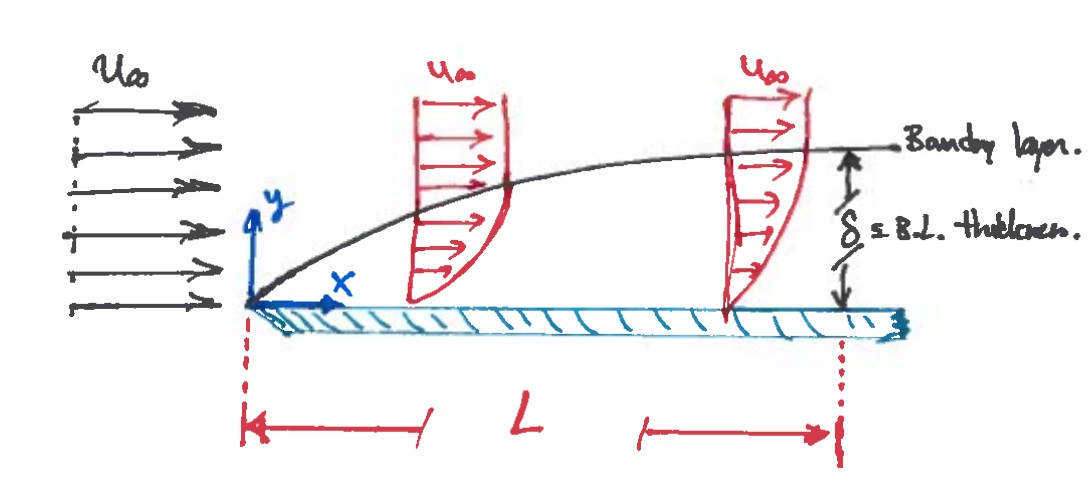
\includegraphics[width=0.5\linewidth]{Lecture Number/Figures/Lecture 6, Jan 30, 2024, Boundary Layer Concept.jpg}
    \caption{Boundary Layer Concept}
    \label{fig:Boundary Layer Concept}
\end{figure}
Assuming that Re$_{l} \gg 1$ and $\delta \ll \ell$, then we can rely on the following normalization factors (order of magnitude analysis).
\begin{table}
    \centering
    \caption{Order of Magnitude Analysis}
    \label{tab:Order of Magnitude Analysis}
    \begin{tabular}{c|ccc}
        & \textbf{Variable} & \textbf{Order of Magnitude} & \textbf{Normalization Factor} \\
        \hline
        Streamline Velocity & $u$ & $u_{\infty}$ & $u = u^* u_{\infty}$ \\
        Streamline Spatial Coordinate & $x$ & $\ell$ & $x = x^* \ell$ \\
        Orthogonal Directional Coordinate & $y$ & $\delta$ & $y = y* \delta$ \\
        Orthogonal Velocity & $v$ & $\mathcal{V}$?? & $v = v* \mathcal{V}$ \\
        \end{tabular}
\end{table}
Let's start with the continuity equation (incompressible flow):
\begin{gather*}
    \frac{\partial u_i}{\partial x_i} = 0 \\
    \frac{\partial u}{\partial x} + \frac{\partial v}{\partial y} = 0 \\
    \frac{\partial u^* u_{\infty}}{\partial x^* \ell} + \frac{\partial v^* \mathcal{V}}{\partial y^* \delta} = 0 \\
    \implies \left(\frac{u_{\infty}}{\ell}\right) \frac{\partial u^*}{\partial x^*} + \left(\frac{\mathcal{V}}{\delta}\right) \frac{\partial v^*}{\partial y^*} = 0 \\
    \implies \frac{\partial u^*}{\partial x^*} +\frac{\mathcal{V} \ell}{u_{\infty} \delta} \frac{\partial v^*}{\partial y^*} = 0 \\
\end{gather*}
Based on the order of magnitude analysis, 
\begin{gather*}
    \frac{\mathcal{V} \ell}{u_{\infty} \delta} = 1 \\
    \implies \mathcal{V} = \frac{u_{\infty} \delta}{\ell} \\
\end{gather*}
Therefore, if $\delta ll \ell$, then $\mathcal{V} \ll u_{\infty}$. This provies that streamline velocity dominates. 

Now, let's move to the Navier-Stokes equation. First, the x-dir:
\begin{gather*}
    \cancelto{\frac{\partial u}{\partial t}}{\text{S.S.}} + u \frac{\partial u}{\partial x} + v \frac{\partial u}{\partial y} = -\frac{1}{\rho} \frac{\partial P}{\partial x} + \nu \left(\frac{\partial^2 u}{\partial x^2} + \frac{\partial^2 u}{\partial y^2}\right) 
\end{gather*}
y-dir:
\begin{gather*}
    \cancelto{\frac{\partial v}{\partial t}}{\text{S.S.}} + u \frac{\partial v}{\partial x} + v \frac{\partial v}{\partial y} = -\frac{1}{\rho} \frac{\partial P}{\partial y} + \nu \left(\frac{\partial^2 v}{\partial x^2} + \frac{\partial^2 v}{\partial y^2}\right)
\end{gather*}

Let's look at the x-dir expression:
\begin{gather*}
    (u^* u_{\infty}) \frac{\partial (u^* u_{\infty})}{\partial (x^* \ell)} + (v^* \mathcal{V}) \frac{\partial (u^* u_{\infty})}{\partial (y^* \delta)} = -\frac{1}{\rho} \frac{\partial P}{\partial (x^* \ell)} + \nu \left(\frac{\partial^2 (u^* u_{\infty})}{\partial (x^* \ell)^2} + \frac{\partial^2 (u^* u_{\infty})}{\partial (y^* \delta)^2}\right) \\
    %---------------------------------------
    \implies \left(\frac{u_{\infty}^2}{\ell}\right) u^* \frac{\partial u^*}{\partial x^*} + \left(\frac{u_{\infty} \mathcal{V}}{\delta}\right) v^* \frac{\partial u^*}{\partial y^*} = -\frac{1}{\rho \ell} \frac{\partial P}{\partial x^*} + \nu \left(\left(\frac{u_{\infty}}{\ell^2}\right) \left(\frac{\partial^2 u^*}{\partial (x^*)^2} + \left(\frac{u_{\infty}}{\delta^2}\right) \frac{\partial^2 u^*}{\partial (y^*)^2}\right)\right) 
\end{gather*}
Using $\mathcal{V} = \frac{u_{\infty} \delta}{\ell}$, 
\begin{gather*}
    \left(\frac{u_{\infty}^2}{\ell}\right) u^* \frac{\partial u^*}{\partial x^*} + \left(\frac{u_{\infty}^2}{\ell}\right) v^* \frac{\partial u^*}{\partial y^*} = -\frac{1}{\rho \ell} \frac{\partial P}{\partial x^*} + \frac{\nu u_{\infty}}{\delta^2} \left(\cancelto{\left(\frac{\delta^2}{\ell^2}\right)}{0} \frac{\partial^2 u^*}{\partial (x^*)^2} + \frac{\partial^2 u^*}{\partial (y^*)^2}\right) 
\end{gather*}
Note the term inside the $\nu$ term is zero since $\delta \ll \ell$. From order of magnitude analysis, we can say
\begin{equation*}
    \text{Scaling of LHS} ~ \text{Scaling of RHS}
\end{equation*}
% i missed this part
% \begin{gather*}
%     \frac{u_{\infty}^2}{\ell} \sim \frac
\begin{gather*}
    \frac{\delta^2}{\ell^2} ~ \frac{\nu}{\ell u_{\infty}} = \frac{1}{\text{Re}}
\end{gather*}
So, if $\delta^2 \ll \ell^2$, then $\frac{1}{\text{Re}} \ll 1$. This implies the flow remains 2D for high Re. 

At this point, we can look at the scaling for pressure,
\begin{gather*}
    \frac{u_{\infty}^2}{\ell} ~ (\text{Pressure Scaling}) \left(\frac{1}{\rho}
    \frac{\partial P}{\partial x} = 0 \left(\frac{\rho u_{\infty}^2}{\ell}\right)\right)
\end{gather*}
Let's apply the same process to the y-direction. The results are:
\begin{gather*}
    \left(\frac{u_{\infty} \mathcal{V}}{\ell}\right) u^* \frac{\partial v^*}{\partial x^*} + \left(\frac{\mathcal{V}^2}{\delta^2}\right) v^* \frac{\partial v^*}{\partial y^*} = -\frac{1}{\rho} \frac{\partial P}{\partial y} + \nu \left(\left(\frac{\mathcal{V}}{\ell^2}\right) \frac{\partial^2 v^*}{\partial (x^*)^2} + \left(\frac{\mathcal{V}}{\delta^2}\right) \frac{\partial^2 v^*}{\partial (y^*)^2}\right) 
\end{gather*}
Since $\delta/\ell \ll 1$ and $u_{\infty} \mathcal{V}/\ell = 0$
\begin{gather*}
    \implies 0 = \frac{1}{\rho} \frac{\partial P}{\partial y^*} 
\end{gather*}
We can see that 
\begin{gather*}
    \text{Scaling of } \frac{\partial P}{\partial y} ~ \frac{u_{\infty}^2 \delta}{\ell^2} \\
    % \frac{\partial P}{\partial x} ~ \rho \frac{\u_{\infty}^2}{\ell} 
\end{gather*}
We can again show that 
\begin{gather*}
    \frac{\partial P}{\partial x} gg \frac{\partial P}{\partial y} 
\end{gather*}